% Compile with: lualatex diffusion_architecture.tex
\documentclass[11pt,a4paper]{article}

% Fonts and encoding
\usepackage{fontspec}
\setmainfont{Latin Modern Roman}
\setmonofont{Latin Modern Mono}

% Core packages
\usepackage{amsmath,amssymb}
\usepackage{booktabs}
\usepackage{xcolor}
\usepackage{listings}
\usepackage{geometry}
\usepackage{hyperref}
\usepackage{tikz}
\usetikzlibrary{shapes.geometric, arrows.meta, positioning, fit, backgrounds, calc}

\geometry{margin=1in}

% Colors
\definecolor{inputcolor}{RGB}{76, 175, 80}
\definecolor{embedcolor}{RGB}{33, 150, 243}
\definecolor{encodercolor}{RGB}{156, 39, 176}
\definecolor{headcolor}{RGB}{255, 152, 0}
\definecolor{outputcolor}{RGB}{244, 67, 54}
\definecolor{condcolor}{RGB}{0, 188, 212}
\definecolor{blockbg}{RGB}{245, 245, 245}
\definecolor{codebg}{RGB}{248, 248, 248}

% Code listing style
\lstset{
    backgroundcolor=\color{codebg},
    basicstyle=\ttfamily\small,
    breaklines=true,
    frame=single,
    rulecolor=\color{gray!30},
    numbers=none,
    showstringspaces=false,
}

\title{\textbf{GETRegionDiffusion Model Architecture}\\[0.5em]
\large A Diffusion Transformer for Genomic Region-Based Masked Motif Prediction}
\author{Architecture Documentation}
\date{\today}

\begin{document}

\maketitle

\section{Overview}

\texttt{GETRegionDiffusion} is a \textbf{Diffusion Transformer (DiT)} adapted for genomic region-based masked motif prediction. It combines the structure of a masked autoencoder with diffusion-style timestep conditioning. The model learns to reconstruct masked genomic motif patterns, conditioned on the diffusion timestep which acts as a noise level indicator.

\section{Architecture Diagram}

\begin{figure}[htbp]
\centering
\resizebox{0.95\textwidth}{!}{%
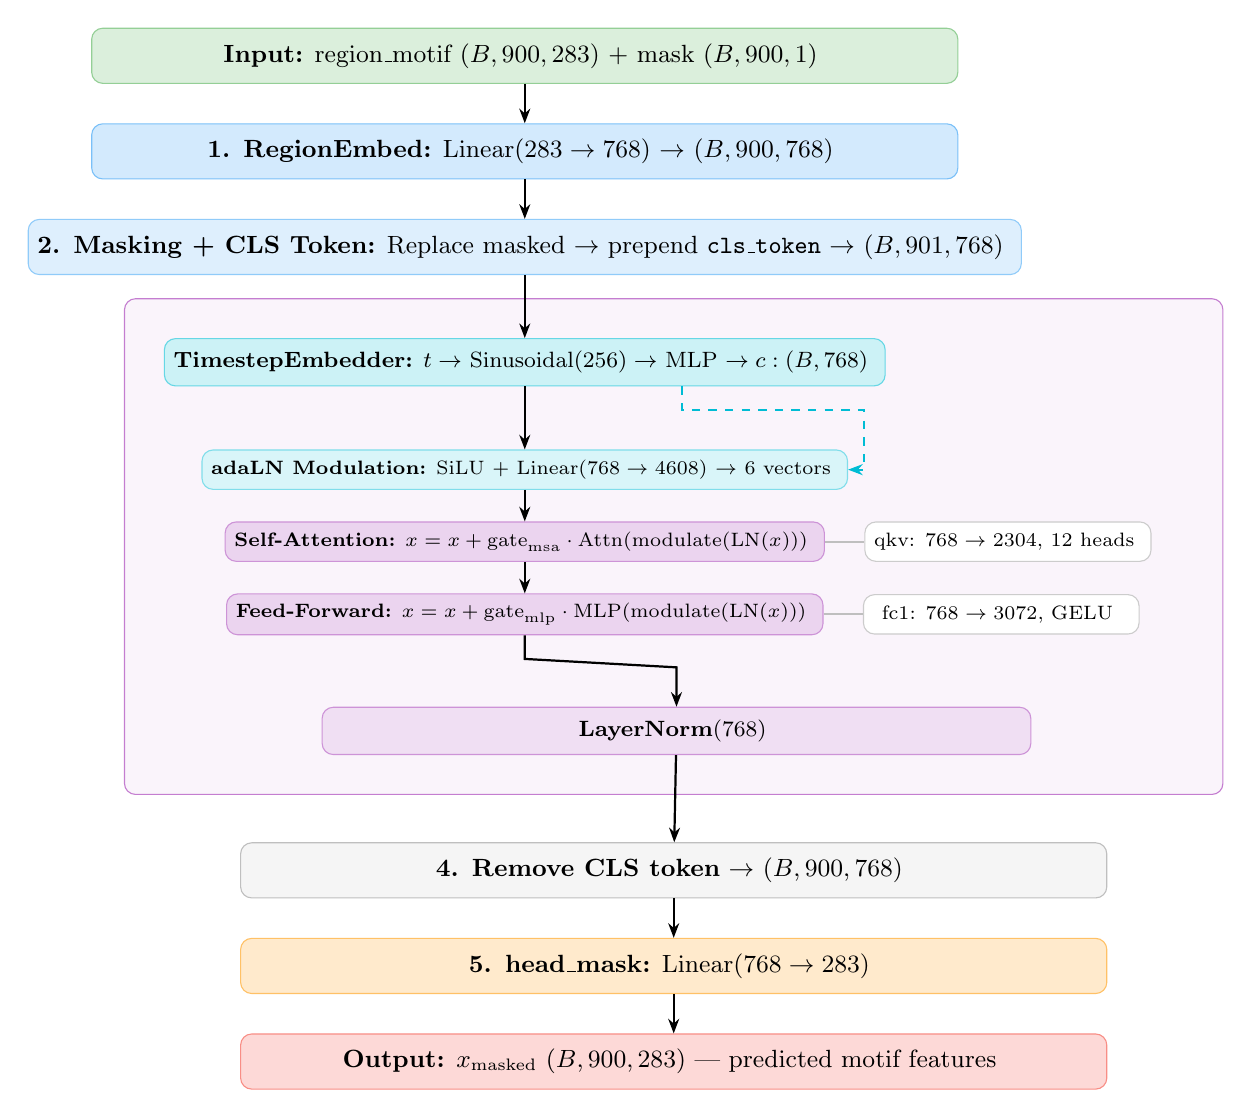
\begin{tikzpicture}[
    node distance=0.5cm,
    block/.style={rectangle, draw, rounded corners, minimum width=11cm, minimum height=0.7cm, align=center, font=\small},
    innerblock/.style={rectangle, draw, rounded corners, minimum width=9cm, minimum height=0.6cm, align=center, font=\footnotesize},
    tinyblock/.style={rectangle, draw, rounded corners, minimum width=7cm, minimum height=0.5cm, align=center, font=\scriptsize},
    detailblock/.style={rectangle, draw, rounded corners, minimum width=3.5cm, minimum height=0.5cm, align=center, font=\scriptsize},
    arrow/.style={-{Stealth[scale=0.8]}, thick},
    dashedarrow/.style={-{Stealth[scale=0.8]}, thick, dashed, condcolor},
    label/.style={font=\footnotesize\bfseries},
]

% ============ TOP SECTION ============
% Input
\node[block, fill=inputcolor!20, draw=inputcolor!60] (input) {
    \textbf{Input:} region\_motif $(B, 900, 283)$ + mask $(B, 900, 1)$
};

% Region Embed
\node[block, fill=embedcolor!20, draw=embedcolor!60, below=of input] (regionembed) {
    \textbf{1. RegionEmbed:} Linear$(283 \rightarrow 768)$ $\rightarrow$ $(B, 900, 768)$
};

% Masking
\node[block, fill=embedcolor!15, draw=embedcolor!50, below=of regionembed] (masking) {
    \textbf{2. Masking + CLS Token:} Replace masked $\rightarrow$ prepend \texttt{cls\_token} $\rightarrow$ $(B, 901, 768)$
};

% ============ ENCODER SECTION ============
% Timestep Embedder (first element inside encoder)
\node[innerblock, fill=condcolor!20, draw=condcolor!60, below=0.8cm of masking] (timestep) {
    \textbf{TimestepEmbedder:} $t \rightarrow$ Sinusoidal$(256) \rightarrow$ MLP $\rightarrow c: (B, 768)$
};

% ============ DiT BLOCK CONTENTS ============
% adaLN
\node[tinyblock, fill=condcolor!15, draw=condcolor!50, below=0.8cm of timestep] (adaln) {
    \textbf{adaLN Modulation:} SiLU + Linear$(768 \rightarrow 4608)$ $\rightarrow$ 6 vectors
};

% Self-Attention
\node[tinyblock, fill=encodercolor!20, draw=encodercolor!50, below=0.4cm of adaln] (attn) {
    \textbf{Self-Attention:} $x = x + \text{gate}_\text{msa} \cdot \text{Attn}(\text{modulate}(\text{LN}(x)))$
};

% MLP Block
\node[tinyblock, fill=encodercolor!20, draw=encodercolor!50, below=0.4cm of attn] (mlp) {
    \textbf{Feed-Forward:} $x = x + \text{gate}_\text{mlp} \cdot \text{MLP}(\text{modulate}(\text{LN}(x)))$
};

% Detail boxes (to the right)
\node[detailblock, fill=white, draw=gray!40, right=0.5cm of attn] (attndetail) {
    qkv: $768 \rightarrow 2304$, 12 heads
};
\node[detailblock, fill=white, draw=gray!40, right=0.5cm of mlp] (mlpdetail) {
    fc1: $768 \rightarrow 3072$, GELU
};

% ============ DiT BLOCK CONTAINER (fit around contents) ============
\begin{scope}[on background layer]
    \node[draw=encodercolor!50, fill=encodercolor!8, rounded corners, 
          fit=(adaln)(attn)(mlp)(attndetail)(mlpdetail),
          inner sep=0.4cm, label={[label, encodercolor!70]north west:{\hspace{0.1cm}DiTBlock $\times$ 12}}] (ditblockbox) {};
\end{scope}

% Final LayerNorm
\node[innerblock, fill=encodercolor!15, draw=encodercolor!50, below=0.5cm of ditblockbox] (finalnorm) {
    \textbf{LayerNorm}$(768)$
};

% ============ ENCODER CONTAINER (fit around all encoder contents) ============
\begin{scope}[on background layer]
    \node[draw=encodercolor!60, fill=encodercolor!5, rounded corners,
          fit=(timestep)(ditblockbox)(finalnorm),
          inner sep=0.5cm, label={[label, encodercolor!80]north west:{\hspace{0.1cm}3. GETRegionDiTEncoder}}] (encoderbox) {};
\end{scope}

% ============ BOTTOM SECTION ============
% Remove CLS
\node[block, fill=blockbg, draw=gray!50, below=0.6cm of encoderbox] (removecls) {
    \textbf{4. Remove CLS token} $\rightarrow$ $(B, 900, 768)$
};

% Head
\node[block, fill=headcolor!20, draw=headcolor!60, below=of removecls] (head) {
    \textbf{5. head\_mask:} Linear$(768 \rightarrow 283)$
};

% Output
\node[block, fill=outputcolor!20, draw=outputcolor!60, below=of head] (output) {
    \textbf{Output:} $x_\text{masked}$ $(B, 900, 283)$ --- predicted motif features
};

% ============ ARROWS ============
% Main flow
\draw[arrow] (input) -- (regionembed);
\draw[arrow] (regionembed) -- (masking);
\draw[arrow] (masking) -- (timestep);
\draw[arrow] (timestep) -- (adaln);
\draw[arrow] (adaln) -- (attn);
\draw[arrow] (attn) -- (mlp);
\draw[arrow] (mlp.south) -- ++(0,-0.3) -- ($(ditblockbox.south)+(0,0)$) -- (finalnorm);
\draw[arrow] (finalnorm) -- (removecls);
\draw[arrow] (removecls) -- (head);
\draw[arrow] (head) -- (output);

% Detail connectors
\draw[gray!50, thick] (attn.east) -- (attndetail.west);
\draw[gray!50, thick] (mlp.east) -- (mlpdetail.west);

% Conditioning arrow (timestep feeds into adaLN)
\draw[dashedarrow] (timestep.south) ++(2cm,0) -- ++(0,-0.3) -| ($(adaln.east)+(0.2cm,0)$) -- (adaln.east);

\end{tikzpicture}
}
\caption{GETRegionDiffusion architecture. The model embeds genomic region motif features, applies masking, and processes through a DiT-style transformer with timestep conditioning via adaptive layer normalization (adaLN). The output head predicts motif features for masked regions.}
\label{fig:architecture}
\end{figure}

\section{Key Components}

\subsection{Adaptive Layer Normalization (adaLN)}

The core innovation from DiT. Instead of standard LayerNorm, the model uses a modulation function:
\[
\text{modulate}(x, \text{shift}, \text{scale}) = x \cdot (1 + \text{scale}) + \text{shift}
\]
where \texttt{shift} and \texttt{scale} are predicted from the timestep embedding. This allows the model to be conditioned on the diffusion timestep.

\subsection{Diffusion Schedule}

Linear noise schedule with the following parameters:
\begin{lstlisting}
diffusion:
  num_timesteps: 1000
  beta_start: 0.0001
  beta_end: 0.02
\end{lstlisting}

During training, a random timestep $t \in [0, 1000)$ is sampled and used to condition the transformer.

\subsection{Masked Prediction Task}

\begin{itemize}
    \item \textbf{Input:} 900 genomic regions, each with 283 motif features
    \item \textbf{Mask ratio:} 50\% of regions are masked
    \item \textbf{Goal:} Predict the original motif features for masked regions
\end{itemize}

\section{Configuration Parameters}

\begin{table}[htbp]
\centering
\caption{Model configuration from \texttt{dit.yaml}}
\label{tab:config}
\begin{tabular}{@{}lll@{}}
\toprule
\textbf{Parameter} & \textbf{Value} & \textbf{Description} \\
\midrule
\texttt{num\_regions} & 900 & Genomic regions per sample \\
\texttt{num\_motif} & 283 & Motif features per region \\
\texttt{embed\_dim} & 768 & Hidden dimension \\
\texttt{num\_layers} & 12 & Number of DiT blocks \\
\texttt{num\_heads} & 12 & Attention heads \\
\texttt{dropout} & 0.1 & Dropout rate \\
\texttt{mask\_ratio} & 0.5 & 50\% of regions masked \\
\texttt{batch\_size} & 8 & Training batch size \\
\texttt{lr} & 0.0001 & Learning rate \\
\texttt{use\_lora} & true & LoRA fine-tuning enabled \\
\bottomrule
\end{tabular}
\end{table}

\section{Layer Details}

\subsection{TimestepEmbedder}

Embeds scalar timesteps into vector representations:
\begin{enumerate}
    \item Sinusoidal positional embedding: $t \rightarrow \mathbb{R}^{256}$
    \item MLP: Linear$(256 \rightarrow 768)$ + SiLU + Linear$(768 \rightarrow 768)$
    \item Output: conditioning vector $c \in \mathbb{R}^{768}$
\end{enumerate}

\subsection{DiTBlock}

Each of the 12 DiT blocks contains:

\begin{table}[htbp]
\centering
\begin{tabular}{@{}ll@{}}
\toprule
\textbf{Component} & \textbf{Details} \\
\midrule
\texttt{norm1} & LayerNorm(768), no affine parameters \\
\texttt{attn} & Self-Attention: qkv Linear$(768 \rightarrow 2304)$, 12 heads, proj Linear$(768 \rightarrow 768)$ \\
\texttt{norm2} & LayerNorm(768), no affine parameters \\
\texttt{mlp} & fc1: Linear$(768 \rightarrow 3072)$, GELU, fc2: Linear$(3072 \rightarrow 768)$ \\
\texttt{adaLN\_modulation} & SiLU + Linear$(768 \rightarrow 4608)$ producing 6 vectors of dim 768 \\
\bottomrule
\end{tabular}
\end{table}

\section{Training Flow}

\begin{enumerate}
    \item Load pretrained checkpoint (\texttt{checkpoint-799.pth}) with weight renaming
    \item Apply LoRA to \texttt{region\_embed} and \texttt{encoder} layers
    \item For each batch:
    \begin{enumerate}
        \item Sample random timestep $t \in [0, 1000)$
        \item Mask 50\% of regions
        \item Forward pass through DiT
        \item Compute MSE loss on masked positions only
        \item Backpropagation + optimizer step
    \end{enumerate}
    \item Metrics: Pearson correlation, MSE, $R^2$ on masked predictions
\end{enumerate}

\section{Loss Function}

The model uses MSE loss computed only on masked positions:
\[
\mathcal{L} = \frac{1}{|\mathcal{M}|} \sum_{i \in \mathcal{M}} \| \hat{x}_i - x_i \|^2
\]
where $\mathcal{M}$ is the set of masked region indices, $\hat{x}_i$ is the predicted motif vector, and $x_i$ is the ground truth.

\end{document}

